%%%%%%%%%%%%%%%%
% INTRODUCTION %
%%%%%%%%%%%%%%%%
\chapter{Introduction}

% TODO: Include a second citation. Include \eg \ie examples. Include references. Include em dash.
Here is the introduction. My dissertation introduces \emph{widgets}. If I wish
to cite someone, I could refer to them in text as in \citet{zongker2006chicken},
or parenthetically \citep{zongker2006chicken}. I can also cite just the
year \citeyearpar{zongker2006chicken} or mention the author,
\citeauthor{zongker2006chicken}.


\begin{quote}
This dissertation template is handy. I like it and use it every time I write a
dissertation.\\
\hspace*{\fill} --- Abraham Lincoln \citeyearpar{zongker2006chicken}
\end{quote}


\section{Stuff}
\label{sec:stuff}

Here is a section on stuff.

\subsection{Artificial Neural Networks}
\label{sec:neuralnet}

See Figure~\ref{fig:neuralnet} for a neural network.

\begin{figure}[th]
	\begin{center}
	   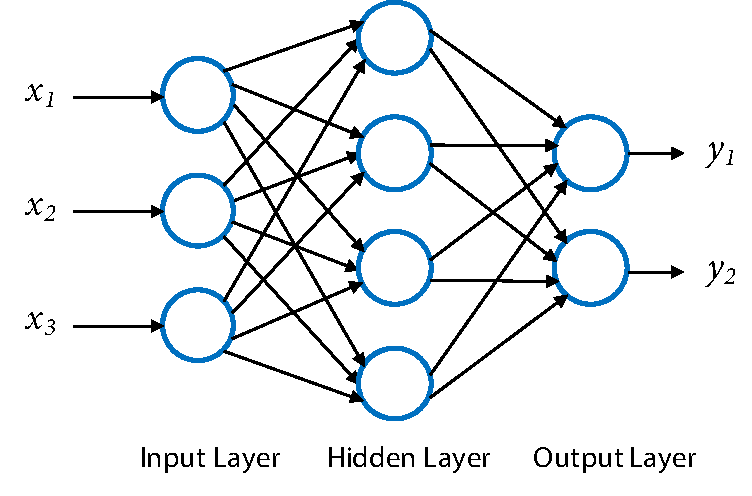
\includegraphics[width=0.8\linewidth]{figures/neuralnet}
	\end{center}
	\caption[An example neural network with two final outputs]
		{An example neural network with two final outputs. Notice how each
		neuron in one layer connects to each neuron in the following layer. This
		is called \emph{fully connected}.}
	\label{fig:neuralnet}
\end{figure}

Cool.
